\documentclass[conference]{IEEEtran}
% \IEEEoverridecommandlockouts

\usepackage{cite}
\usepackage{amsmath,amssymb,amsfonts}
\usepackage{algorithmic}
\usepackage{graphicx}
\usepackage{textcomp}
\usepackage{xcolor}
\usepackage{tabularx}
\usepackage{array}
\usepackage{subcaption}
\usepackage{booktabs}
\usepackage{multirow}
\usepackage{hyperref}
\usepackage{listings}


\newcolumntype{Y}{>{\raggedright\arraybackslash}X}
\lstset{
  basicstyle=\ttfamily\scriptsize,
  breaklines=true,
  breakatwhitespace=false,
  columns=fullflexible,
  keepspaces=true,
  showstringspaces=false,
  literate={≤}{{$\leq$}}1
}

\def\BibTeX{{\rm B\kern-.05em{\sc i\kern-.025em b}\kern-.08em
    T\kern-.1667em\lower.7ex\hbox{E}\kern-.125emX}}
    
\begin{document}

\title{Supporting Materials\\}

\section{Introduction}

These supporting materials accompany the research paper
\emph{Extract, then decide: a two-stage pipeline to identify seizure 
frequency in epilepsy clinic letters}.

It contains four sections: an extended literature review; a 
description of the project life cycle (planning, development, 
implementation, testing, and evaluation); the tools used 
to build and run the system; and a critical appraisal of 
design decisions, lessons learned, and the outcome with 
hindsight.

\section{Extended Literature Review}

\subsection{Complexity of Clinical Narratives}

Clinical letters use narrative language so that clinicians can 
record the patient's situation, their judgement, and their 
uncertainty. That flexibility improves clinical communication, 
but it makes the information difficult to use at scale~\cite{b1}. 
Clinicians often use hedging to describe certainty, frequency, 
and quantity rather than stating a precise value~\cite{b2}. 
The task of information extraction (IE) is to convert that
nuanced information into a standardised form while
preserving its essential meaning.

Epilepsy clinic letters illustrate that complexity. One letter 
can contain diagnoses, prescriptions, history, seizure 
descriptions, and several references to seizure frequency. 
Fonferko-Shadrach \emph{et al.} report much lower human 
agreement for seizure frequency (per-item F1 = 0.47) than 
for prescriptions (0.87) or diagnoses (0.83)\cite{b3}. They 
attribute this to the variety of frequency expressions and to 
mentions of more than one seizure or event type. 
Effective extraction requires clearly defined policies and
procedures describing what to extract and how to 
represent it.

\subsection{Seizure Frequency as a Selection Task}

The same letter can be used for different purposes. 
ExECT and the later annotation study treat it as 
an inventory: they record several entity mentions and 
their attributes. One letter may list several anti-seizure 
medications, each with a name, dose, unit, and 
administration frequency~\cite{b4,b3}. That form is 
appropriate when the aim is building a broad clinical
inventory.

The task in this study is different. Gan \emph{et al.} 
assign each letter one label for the patient's current 
seizure frequency status~\cite{b5}. The system has to gather 
candidate descriptions, interpret their meaning and 
time frame, and choose the single normalised label 
that best represents the current pattern. Earlier 
one-label studies use the same formulation~\cite{b6,b7,b8}. 
The single label extraction implies that it is all one 
task, but this study proposes two separate stages: 
extracting every candidate with its evidence in a 
canonical form, then deciding the final answer from 
those candidates.

Two common cases show why that split matters. 
Diary-style counts may need to be combined: \emph{1 in June, 
0 in July, 2 in August} can become \texttt{3 in 3 months}. 
Competing statements may instead require precedence: 
\emph{She may remain seizure-free for up to 4 months, but 
then will experience clusters of 5 seizures in a single day.} 
Different annotation guidelines would record those cases 
differently. Separate stages make the policy choice 
inspectable rather than implicit.

\subsection{Rules, Fine-Tuned Models, and LLMs}

Several papers have published seizure frequency 
extraction systems using rules, fine-tuned models, or 
prompted large language models. Rules match terms 
and apply domain logic. ExECT does this for a clinical 
inventory; Decker \emph{et al.} use regular expressions 
for seizure-related variables~\cite{b4,b9}. Fine-tuned 
BERT models learn the mapping from labelled examples, 
as in Xie \emph{et al.} and Fernandes \emph{et al.}~\cite{b6,b10}. 
Table~\ref{tab:historical} lists the F1 scores those studies 
report. The scores are not a ranking of methods: each 
study uses its own dataset, label set, and evaluation.

\begin{table}[!t]
\caption{Past seizure frequency papers: headline results}
\label{tab:historical}
\centering
\begin{tabularx}{\linewidth}{Ycll}
\toprule
\textbf{Author} & \textbf{Year} & \textbf{Method} & \textbf{F1 score} \\
\midrule
Xie et al. & 2022 & Fine-tuned BERT & 0.83 \\
Decker et al. & 2022 & Rules & 0.82 \\
Fonferko-Shadrach et al. & 2024 & Rules & 0.66 \\
Fernandes et al. & 2024 & Fine-tuned BERT & 0.37 \\
Holgate et al. & 2024 & Prompted LLM & 0.73 \\
Holgate et al. & 2025 & Fine-tuned LLM & 0.68 \\
Gan et al. & 2026 & Fine-tuned LLM & 0.79 \\
\midrule
Brown \& Gan & 2026 & Hybrid & 0.80 \\
\bottomrule
\end{tabularx}
\end{table}

Prompted and fine-tuned LLMs are more recent. 
Holgate \emph{et al.} show that a prompted model can 
extract seizure information from instructions and 
examples~\cite{b7}. Holgate \emph{et al.} 
and Gan \emph{et al.} later fine-tune models to a defined 
output format~\cite{b8,b5}. 

BERT-style encoders and decoder-based LLMs 
share the transformer architecture. The practical 
difference is in-context learning: an LLM can 
follow instructions and examples without 
task-specific training~\cite{b11}. That behaviour 
transfers to clinical extraction, where clear 
instructions and examples can reduce the need for 
heavy post-processing~\cite{b12}. Gan \emph{et al.}
show that combining structured prompting and 
fine-tuning can deliver even stronger performance. 
This study explores whether structured
prompting in a two-stage pipeline can deliver 
comparable performance to a fine-tuned LLM.

\subsection{Modular and Sequential Extraction Pipelines}

Multi-stage clinical extraction pipelines split a task 
into distinct stages instead of asking a model for 
one final answer in a single step. CLINES uses 
stages for chunking, extraction, attribute assignment, 
normalisation, date resolution, and aggregation~\cite{b14}. 
Seizure frequency studies have also decomposed 
the task in structured prompting including numbered 
reasoning steps and summarise-then-extract 
designs~\cite{b7,b15}. 

This study decomposes the task into two stages: 
extracting candidate evidence into a structured 
record, and deciding the final answer from that 
record. One LLM call performs the extraction. The 
decision stage can be performed by rules or a second LLM 
call, so the two methods can be compared with the 
extraction held fixed. Past research on seizure 
frequency gives rules a minor repair role after an 
LLM; this study evaluates whether they can play
a more substantial role in post-processing.

\section{Planning}

The project lifecycle is divided into five stages:
planning, development, implementation, testing and
evaluation. The sections below describe the key
decisions, the rationale behind them, and the
sources they were based on.

There are two key documents in the planning 
phase: 

\begin{enumerate}
\item The project brief, created by my supervisor.
\item The problem specification and project plan, 
created by me.
\end{enumerate}

\subsection{Project Brief}

The project brief outlines the initial scope of the
project. The problem specification and project
plan refines the scope, specifies the research 
objectives and describes the methods used to
achieve them. The project brief was:

\begin{quote}
Instead of training models, this project builds a 
training-free (or minimal-training) multi-agent 
extraction system that reads epilepsy letters and 
outputs structured fields (e.g., ASM, seizure 
type/frequency, investigations, epilepsy 
syndrome/type). The student will design roles 
such as: (a) Section/Timeline Agent (segments 
text, builds timeline), (b) Field Extractor Agents 
(one per field group), (c) Verification Agent 
(checks evidence spans, contradictions, 
missingness), and (d) Aggregator Agent 
(produces final JSON + confidence + citations 
to text spans). The key research goal is 
reliability: compare single-prompt extraction 
vs multi-agent extraction under the same 
budget constraints, and test improvements 
from self-consistency, evidence requirements 
(“answer only if supported by quote”), and 
structured output validation. Evaluation uses 
field-level accuracy/F1,  and robustness tests. 
Data can be synthetic or de-identified samples 
if available. Deliverables: an end-to-end agentic 
pipeline, evaluation harness, and a dissertation 
focused on engineering + empirical study of 
reliability.
\end{quote}

The deliverables are a narrow specification of
what a successful project would look like:

\begin{enumerate}
\item An end-to-end agentic pipeline.
\item An evaluation harness.
\item A dissertation focused on engineering + empirical study of reliability.
\end{enumerate}

The type of data this would be applied to was
narrowly defined as epilepsy letters, but it
was undetermined whether the specific data 
source was synthetic or de-identified samples. 
This was one key decision to be agreed 
in the project kick-off meeting.

The research would compare a single-prompt
extraction vs. multi-agent extraction, and the
multi-agent system included a number of 
initial suggestions such as verification agent
and aggregator agent. The precise 
implementation of the multi agent system would be
defined as the research progresses, guided by best 
practices in the literature and the results from 
empirical experiments.

In the initial project kick-off meeting it was 
agreed that the specific data source used
would be a set of 1,500 synthetic clinical 
letters that the supervisor had access to. 
As these were synthetic letters, there would
be no need to get specific ethics approval 
to use for research purposes. 

\subsection{Problem Specification and Project Plan}

The problem specification and project plan was 
uploaded to the university Canvas site on the
5$^{th}$ June 2026. This is a direct extract 
from the methods section:

\begin{quote}
\vspace{0.2em}
There are two primary data sources in this project:

\vspace{0.2em}
\begin{itemize}
\item 1,500 synthetic clinical letters and structured labels from Gan \emph{et. al} \cite{b5}
\item 200 synthetic clinical letters and structured labels from Fonferko-Shadrach \emph{et. al}\cite{b3}
\end{itemize}

\vspace{0.2em}
The project will use LLMs as the core AI tool, using both open (e.g. Qwen 3.6) and closed
(e.g. GPT 5.4) models. The research will involve building an agent harness around the
model that enables it to ingest clinical letters and prompt instructions, produce a
structured output, and have that output validated and evaluated.

\vspace{0.2em}
The research will be empirical in nature and focus primarily on assessing the quality,
reliability and validity of the outputs. Cost, latency, data schema complexity and
evidence specificity will be key experimental variables tested.

\vspace{0.2em}
Evaluation will take place in three key forms: comparing the accuracy (F1 score) of the
outputs vs. the ground-truth labels from the two data sources, assessing the validity of
the structured data schema created, and assessing the validity of the evidence cited. A
series of ablations will be conducted to isolate the impact of different components of
the agent harness.

\vspace{0.2em}
The F1 score evaluated on a set of ground-truth labels is the de-facto standard for
evaluating AI models on how well they can complete a classification task. Evaluating
the model on two different datasets optimised for two different tasks effectively tests
the flexibility of the system. 

\end{quote}

The ExECTv2 dataset \cite{b3} was used extensively
as per the original plan. The pipeline was built, 
experiments were conducted and results were analysed in 
depth and benchmarked against the prior results. 
However, when the time came to write the paper
it became clear that writing about two datasets
with different annotation policies, evaluation measures,
error profiles and sample sizes required the reader
to hold too much information in mind. 

As a result, the empirical analysis in the paper and the 
primary evaluation in these materials focus on the 
seizure-frequency extraction task on the Gan letters. 
ExECTv2 appears here only as design history and as the 
descriptive inventory panel in 
Section~\ref{sec:inventory-feasibility}. We used the 
pipeline built for ExECTv2 to extract diagnoses, medications
and investigations from the main dataset of 1,500
synthetic letters as that feasibility study; some of the 
design choices for the seizure-frequency extraction
pipeline are directly informed by designing a modular
system that can be applied to both tasks. Results 
benchmarked against the ExECTv2 dataset will
be published in a separate paper.

The following sections describe how the rest of this 
plan was implemented.

\section{Development}

This section explains how the initial project proposal was 
translated into a focused and testable research approach. 
It records the evidence, design choices, and trade-offs 
that led to the final method.

\subsection{Original Design Requirements}

The original brief contained a series of key design 
requirements for the pipeline. It must:

\vspace{0.2em}
\begin{enumerate}
\item Ingest epilepsy letters
\item Output validated structured fields 
\item Contain verified evidence citations
\item Produce this in an aggregated JSON
\end{enumerate}
\vspace{0.2em}

These design requirements were tightly coupled to a 
multi-agent framework, e.g using a \emph{Verification Agent} 
to check evidence spans and an \emph{Aggregator Agent}
to produce the final JSON and citations. 

The literature review showed that multi-agent systems
are particularly useful for complex tasks \cite{b25},
especially on long-context tasks \cite{b26}. 
However, research also shows that single-agent systems
are often as effective when they are given equal compute 
and multi-agent systems create new failure modes 
as errors propagate throughout the system\cite{b26}.

For this task, the full epilepsy letter and instructions 
fit comfortably in the LLM's context window so there
is no need for convoluted multi-hop pipelines or 
document splitting that multi-agent systems 
performed particularly well on\cite{b14}. Thus, a 
multi-agent system can not be justified on that basis.

It is less clear whether this task is sufficiently complex
to justify a multi-agent system. Past research has 
shown that LLMs struggle with temporal logic and 
numerical logic, and both occur in this task. It is
also a task that human annotators struggle to do
reliably and consistently\cite{b3}. This suggests the task 
is at least somewhat complex and a multi-agent
system is justified on that basis.

However, it is important that each LLM call is given
a sufficiently complex task to justify the added system
complexity. A key research objective is to design 
a reliable system. A reliable system is one that 
contains the minimum amount of complexity 
necessary to function. More components create 
more failure modes, and in a sequential 
process those errors propagate and multiply at 
each step. 

\subsection{Deterministic Code for Deterministic Tasks}

A key design choice early on was to simplify. Any
task that can be reliably completed by a deterministic
system (code) instead of a probabilistic system (LLMs)
should be done deterministically. 

Evidence verification and schema validation are two 
tasks that code can do reliably and efficiently. Initial 
experiments showed that LLMs can not do this task 
reliably; they introduce as many new schema errors 
as they repair, and they occasionally miss invalid 
evidence. Even if they could do the task
reliably, code already does it at a lower
cost and latency. 

Therefore a dedicated \emph{Aggregator Agent} to produce
the final JSON with text citations and a dedicated 
\emph{Verification Agent} to check evidence spans were 
removed from the design after initial experiments.
A \emph{Field Extractor} agent was no longer relevant as 
the task was limited to a single field, seizure 
frequency. Initial experiments showed that a 
\emph{Section/Timeline Agent} was a net-negative 
contribution because correct seizure frequency 
references were not always in the dedicated 
seizure frequency section, and splitting up the 
text encouraged the LLM to select wrong answers
more frequently.

\subsection{Pipeline Design Review}

After initial experiments, all four of the original
proposed LLM agents had been ruled out because
they were now either invalid or empirically performed
worse than a single LLM. This led to a major review
of the pipeline design. 

Comprehensive error analysis showed that the LLM
was consistently finding valid seizure frequency
patterns, providing exact evidence from the text
and often choosing defensible answers based 
on the instructions. It did not need another LLM call to
check its evidence or structure it into JSON; it 
needed cleaner task separation. 

The work separates two clinical operations: extracting 
every relevant mention of seizure frequency from the 
letter, already written in the form the gold-standard 
labels expect, and applying a policy to choose which 
label matches the gold-standard answer. The
labelling conventions and policy choices in the 
gold-standard evidence are valid, but they are not
the only valid choice. Therefore a key pipeline 
requirement is producing results that conform to 
an explicit set of subjective choices. 

The original brief separated mechanical tasks 
across multiple LLM calls; one call splits the 
evidence, another checks the evidence, another 
aggregates it together. With simplicity and 
efficiency in mind, it would be preferable if a 
single LLM call could do all of those tasks at once. 
This would require the LLM to generate a much richer 
intermediate schema. Rather than extracting a single 
seizure frequency label, the LLM would extract
every relevant seizure frequency pattern as 
a distinct entity in a nested JSON, with exact
evidence for every entity, and make an initial 
proposal. 

Using this richer schema, a second LLM call 
could then review the evidence and apply the correct 
policy in hard cases. This reframes the decomposition 
around clinical tasks (extract the candidates, then 
decide between them) instead of mechanical tasks. The 
richer record also makes it possible for deterministic 
rules to apply the same policy to the evidence the LLM 
extracted.

Past research shows that deterministic code
can reliably normalise seizure frequency values,
and hybrid LLM and rules systems can outperform
LLMs alone. Rules-based systems 
struggled with seizure frequency extraction more
than medications, but they still performed better
than human experts. Deterministic code already
performed schema validation and evidence 
verification more reliably than LLMs, so there was 
a case for more deterministic code in the pipeline.

\subsection{Final Pipeline Design}

The final outcome of this design review was a 
pipeline with two stages, 
\texttt{extract} and \texttt{decide}. \texttt{Extract} 
finds all seizure frequency patterns in the letter, 
records each one with a normalised label and
the exact quote supporting it, and selects the
one that best represents the patient's seizure
frequency pattern with a one sentence rationale.
\texttt{Decide} reviews that evidence against 
the established policy and decides whether to
keep, change or revise the provisional answer.

This study's core comparison holds the extraction call 
fixed and changes only who performs \texttt{decide}: 
rules (\texttt{Hybrid}) or a second LLM call 
(\texttt{LLM-only}). 

The original project brief required a pipeline that
could ingest epilepsy letters, output validated 
structured fields, contain verified evidence citations
and produce this in an aggregated JSON. It required
an evaluation harness and a dissertation focused 
on engineering and an empirical study of reliability.
The evaluation section demonstrates all of this.

\section{Implementation}

The implementation was designed to produce a structured, 
reproducible account of current seizure frequency from 
a clinical letter, while retaining the evidence and 
intermediate choices needed to inspect how an answer 
was reached. It describes the reusable pipeline and the 
controlled comparison design; performance results and 
the findings of individual ablations are reported in the 
evaluation section.

\subsection{Structured Record}

The pipeline receives a synthetic clinical letter as input
and produces a structured seizure frequency record. The 
final record contains the submitted frequency label, direct 
supporting evidence, and the metadata needed to identify 
the method, model configuration, data split, and scoring 
policy used. This design makes the final answer usable for 
benchmark evaluation without reducing the whole process 
to an opaque single-label extraction.

The pipeline uses a richer intermediate record than the 
final benchmark label. During extraction, it can retain 
multiple candidate seizure frequency events, their source 
spans, raw wording, time information, and an initial 
proposed answer. This is important because a letter 
may contain several plausible statements: historical 
and current rates, periods without seizures, isolated 
breakthrough events, clusters, and uncertain or 
qualitative descriptions. Preserving the alternatives avoids 
losing information before the annotation policy has been 
applied.

\subsection{Extract and Decide}

The record distinguishes the source wording from the 
canonical label form and from the final answer. The 
\texttt{decide} stage can revise the provisional 
answer while retaining the evidence on which 
the original proposal was based. The final output is 
validated against the expected schema, while source 
data and raw model output are retained separately 
from format repair and clinical policy decisions.

The interface between the two stages is fixed. 
\texttt{Extract} receives the full letter and returns the 
candidate record: every seizure frequency event with its 
quoted span, category and canonical label, plus a 
provisional answer. \texttt{Decide} receives that record 
and the decision policy, and returns the 
final label with the event(s) that support it. In 
\texttt{Hybrid}, the decision rules also rewrite any 
label the model left in a non-canonical form.

\subsection{Rules and Deterministic Components}

Deterministic components implement tasks for which explicit, 
reproducible handling is appropriate. These include parsing 
and schema repair, validation of required evidence fields, 
aggregation of the final record, and rules for normalising 
frequency expressions into the task's closed vocabulary. The 
implementation keeps format-only repair, benchmark 
representation, and clinically meaningful policy rules distinct 
so that a change to one does not silently alter another.

In \texttt{Hybrid}, recorded rules perform the decision 
role. Their authority is recorded by rule type: whether a 
rule merely standardises a label form (dialect or 
form), rewrites the submitted label from the extracted 
evidence (e.g. totalling a seizure diary), or chooses a 
different already-extracted event. No decision 
rule scans the letter for a new candidate. This makes 
deterministic processing an explicit part of the method 
rather than unreported post-processing. 

\subsection{LLM Components}

The LLM implementation uses structured prompts that 
ask the model to return a record containing candidate 
seizure-frequency events, evidence, and a proposed 
answer. The extraction call reads the letter and returns 
that record. In \texttt{LLM-only}, a second call receives 
the record and adjudicates between competing candidates 
under the same policy that the rules apply, written as 
instructions with worked examples. 

The prompt at the end of this document is the template sent to the 
model: task, instructions, allowed label forms, event schema 
and decision schema. The four components ablated in the 
accompanying paper map onto it as follows: the \emph{instructions} are the 
task and instruction blocks; the \emph{examples} are the 
worked examples inside the instructions; the \emph{allowed 
labels} are the closed \texttt{label\_forms} block; and the 
\emph{evidence obligation} is the evidence fields of the event 
schema together with the exact-quote instruction. The letter 
is attached at run time as \texttt{note\_text} and is omitted 
here. Event categories are listed in Table~\ref{tab:event-categories}, 
label forms in Table~\ref{tab:label-forms}, and short decide 
examples in Table~\ref{tab:select-policy}.

\begin{table}[!t]
\caption{Seizure frequency label forms}
\label{tab:label-forms}
\centering
\begin{tabularx}{\linewidth}{lY}
\toprule
\textbf{Family} & \textbf{Written forms} \\
\midrule
Rate &
$N$ per unit;
$N$ per $N$ unit;
$N$ per $N$ to $N$ unit;
$N$ to $N$ per unit;
$N$ to $N$ per $N$ unit;
multiple per unit;
multiple per $N$ unit;
$N$ per multiple unit \\
Cluster &
cluster per unit, $N$ per cluster;
cluster per unit, range per cluster;
cluster per unit, multiple per cluster \\
Seizure free &
seizure free for a duration \\
Unknown &
unknown;
no seizure frequency reference \\
\bottomrule
\end{tabularx}
\end{table}

\begin{table}[!t]
\caption{Seizure frequency event categories in the extraction record}
\label{tab:event-categories}
\centering
\begin{tabularx}{\linewidth}{lY}
\toprule
\textbf{Category} & \textbf{Use} \\
\midrule
\texttt{frequency\_rate} & A countable or range rate \\
\texttt{cluster\_frequency} & How often clusters occur \\
\texttt{seizure\_free} & A seizure-free statement \\
\texttt{last\_event\_only} & A dated last event without a rate \\
\texttt{unknown\_frequency} & Seizures discussed, no usable rate \\
\texttt{no\_reference} & No usable frequency evidence \\
\bottomrule
\end{tabularx}
\end{table}

\begin{table}[!t]
\caption{Decision stage examples}
\label{tab:select-policy}
\centering
\begin{tabularx}{\linewidth}{YYY}
\toprule
\textbf{Events} & \textbf{Provisional answer} & \textbf{After decide} \\
\midrule
3 in March; 6 in May &
\texttt{6 per month} &
\texttt{9 per 3 month} \\
Last seizure on 12th March; well 3 weeks &
\texttt{seizure free for 3 week} &
\texttt{1 per month} \\
\bottomrule
\end{tabularx}
\end{table}


\section{Testing}

A test suite was built to check that letters and gold labels 
loaded without silent changes, that development and held-out 
letters stayed apart, and that work on prompts and rules used 
only the development set. Held-out results were reported only 
as totals. The same suite kept a short list of known hard 
cases: adding up a seizure diary, not counting the same 
evidence twice, handling empty months, reading clusters, and 
preferring the current rate over an older one. When a prompt 
or rule changed, those cases were re-run so a local fix did 
not break earlier behaviour. End-to-end checks confirmed that 
extract then decide still wrote a valid record.

After the package was released, my supervisor installed 
it on the university high-performance computing cluster and 
ran both methods on a new dataset. Both runs finished 
and wrote structured output. That shows the package can be 
installed and used in other environments.

\section{Evaluation}

This section evaluates whether the verified pipeline met the 
research objective: to extract a patient's current seizure 
frequency burden from a clinical letter reliably, with a 
structured evidence record and a reproducible comparison 
between rules and LLMs. The accompanying paper reports the 
headline held-out comparison: on one shared Gemini extract 
record, \texttt{Hybrid} reaches 0.86 Purist and 
\texttt{LLM-only} 0.85. This section expands contract 
adherence, prompt-mechanism 
detail, secondary decompositions, generalisation, and 
evidence-quality limits.

\subsection{Independent real-letter comparison}

DeepSeek V4 Flash was evaluated on Gan 
\emph{et al.}'s Real(300) held-out clinic letters\cite{b3} and demonstrated
the method transfers to real patient data and result patterns hold.
\texttt{Hybrid} remained ahead of \texttt{LLM-only} (0.80 vs.\ 
0.77) and matched the best published synthetic-trained fine-tune 
on the same letters (0.79)\cite{b5}. Results are shown in 
Table~\ref{tab:real-letters}.

\begin{table}[!t]
\caption{Purist micro-F1 on synthetic and real clinic letters}
\label{tab:real-letters}
\centering
\footnotesize
\begin{tabularx}{\linewidth}{Yrrr}
\toprule
\textbf{Method} & \textbf{Synthetic dev} & \textbf{Synthetic test} & \textbf{Real letters} \\
\midrule
Hybrid & 0.83 & 0.82 & 0.80 \\
LLM-only & 0.78 & 0.77 & 0.77 \\
\bottomrule
\end{tabularx}
\end{table}

\subsection{Extracting multiple candidates with exact evidence}

A key feature of the pipeline is the rich extraction record. 
The model is asked to extract every seizure frequency pattern 
in the text, quote an exact evidence span for each, write each 
in a canonical form, and propose which best represents the 
patient's current status. That record is what allows the 
second LLM call in \texttt{LLM-only} and the rules in 
\texttt{Hybrid} to re-use the evidence and improve on the 
provisional answer by +0.06 to +0.07. The cost is a more 
complex schema, and this is where the local models fall 
slightly behind.

The gold standard records one label and one quote per letter. 
The extraction record holds more: on \texttt{test450}, Gemini 
extracted 985 events over 450 letters (2.19 per letter) and 
the six models ranged from 2.19 to 2.82 events per letter. 
The record therefore preserves 
alternatives that a one-label output would discard.

Table~\ref{tab:adherence-supp} shows each model's adherence 
to the extraction schema on \texttt{test450}. The four hosted 
models quoted an exact 
substring of the letter for the selected event in 99\% or more 
of letters; Qwen (97\%) and Gemma (93\%) occasionally 
paraphrased. Gemma also needed the most non-semantic format 
repair (15 letters), typically doubled braces or quotation 
marks that broke the nested JSON, and left 8 letters 
unparsed after repair; those letters are scored as incorrect. 
Format repair is recorded separately from every semantic 
rule and never changes a label.

\begin{table*}[!t]
\caption{Six models as the extraction call on \texttt{test450}: scores and contract adherence (Hybrid)}
\label{tab:adherence-supp}
\centering
\footnotesize
\begin{tabularx}{\textwidth}{Yrrrrrrr}
\toprule
\textbf{Model} & \textbf{Purist} & \textbf{Prag.} & \textbf{Exact evidence} & \textbf{Repairs} & \textbf{Unparsed} & \textbf{Retry rej.} & \textbf{Events} \\
\midrule
Gemini 3.7 Flash & 0.86 & 0.88 & 99.8\% (449) & 0 & 1 & 0 & 985 \\
Grok 4.6 & 0.85 & 0.89 & 100\% (450) & 0 & 0 & 0 & 1063 \\
DeepSeek V4 Flash & 0.82 & 0.85 & 99.6\% (448) & 2 & 0 & 0 & 1267 \\
GPT-5.6 Luna & 0.79 & 0.82 & 98.9\% (445) & 0 & 1 & 0 & 1102 \\
Qwen 3.8 27B & 0.76 & 0.81 & 96.7\% (435) & 3 & 2 & 0 & 1004 \\
Gemma 4 26B & 0.72 & 0.77 & 92.9\% (418) & 15 & 8 & 7 & 1068 \\
\bottomrule
\end{tabularx}

\vspace*{2pt}
\begin{minipage}{\textwidth}
\raggedright\footnotesize
Exact ev.: the quoted span for the selected event is an exact substring of the letter. Repairs: letters needing a non-semantic JSON dialect repair. Unparsed: no valid record after repair. Retry rej.: format-only retries whose output was rejected. Events: extracted events over 450 letters. Source: \texttt{paper\_experiments/gan/rungs/\{model\}/test450/comparison.json}.
\end{minipage}
\end{table*}

\subsection{Development vs.\ test results}

Figure~\ref{devtest} shows the two methods on 
both splits. \texttt{Hybrid} scores 0.87 on 
development and 0.86 on the held-out set, a 
generalisation gap of $-$0.01. \texttt{LLM-only} scores 0.85 
on both. Neither method was tuned on 
held-out letters; prompts and rules were fixed on the 
development split and replayed once. The small gaps are 
consistent with the extraction call doing the pattern 
matching across the whole letter and the decision stage 
acting only on the refined record. The development-only 
rules-extraction baseline mentioned in the Development 
section showed the larger development-to-test drop typical of 
rules tuned on one corpus; it is not part of this comparison 
and is recorded in the repository.

\begin{figure}[t]
    \centering
    
\includegraphics[width=\linewidth]{development_vs_test_generalization.pdf}
     \caption{The two methods on the development and held-out splits, Purist micro-F1. Both share the same extraction call. \texttt{Hybrid} moves from 0.87 to 0.86; \texttt{LLM-only} is 0.85 on both.}
    \label{devtest}
\end{figure}

\subsection{Error examples}

The accompanying paper's residual reading concentrates on 
incorrect \texttt{unknown} answers. The figures below are 
development mechanism illustrations of that mode 
(seizure-free, frequent, and infrequent gold labels each 
submitted as unknown). They explain how competing temporal 
readings and labelling conventions produce the error.

\begin{figure*}[t]
        \centering
        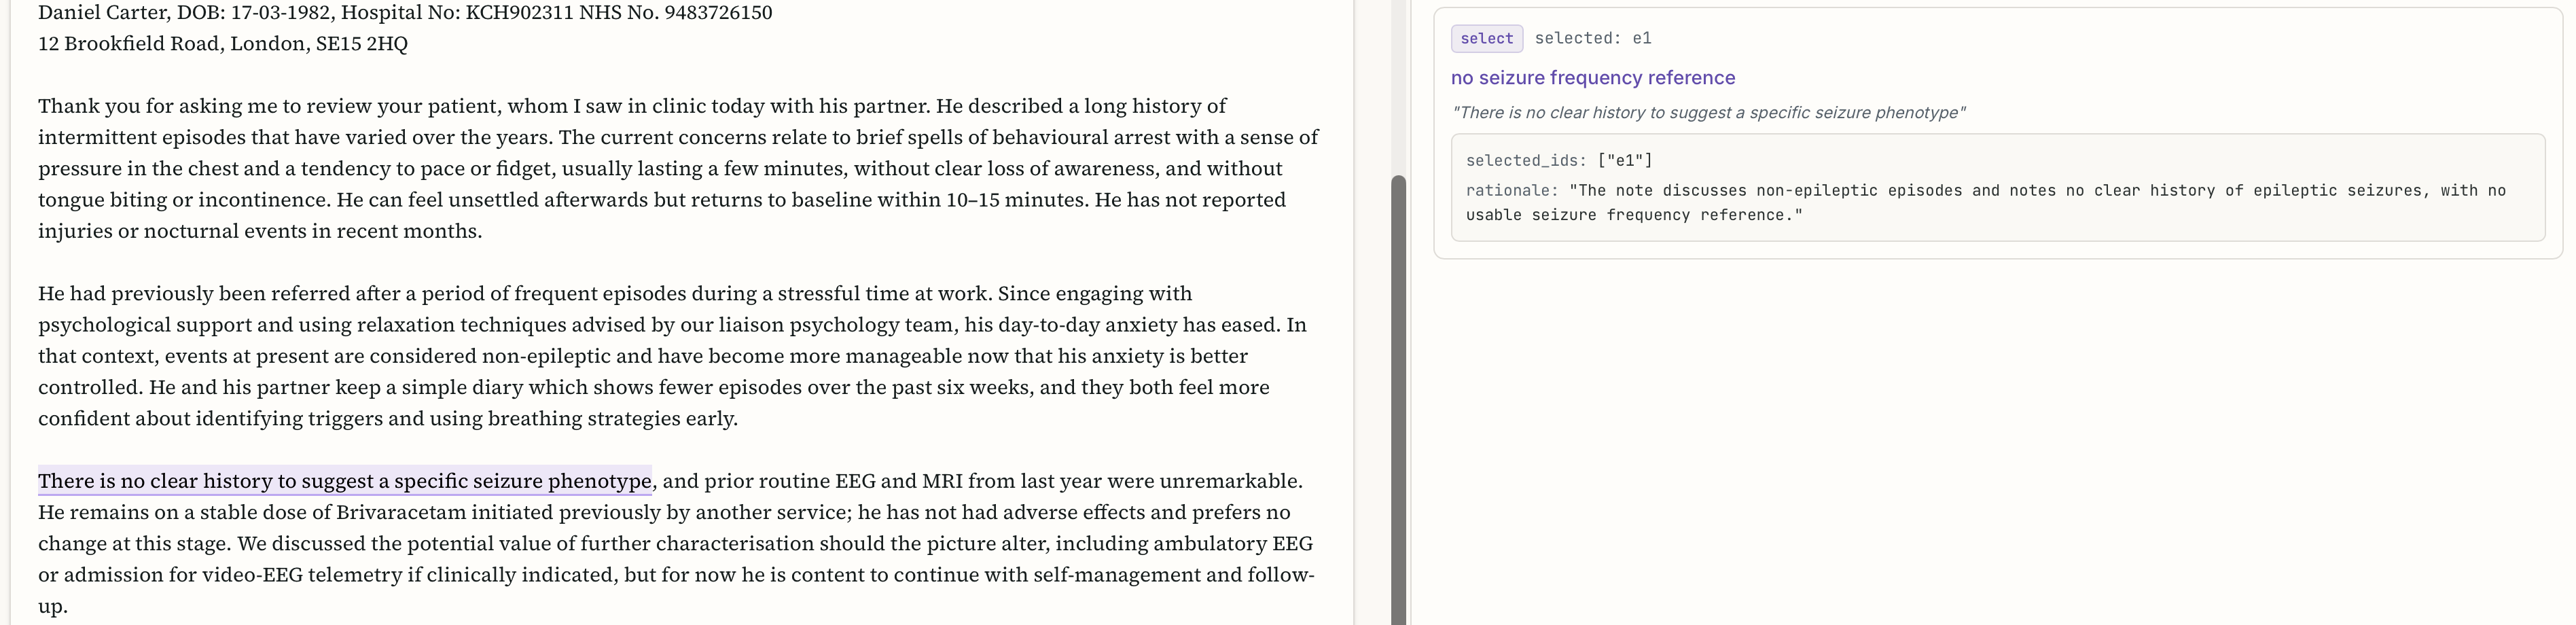
\includegraphics[width=\linewidth]{seizure_free_unknown}
        \caption{Seizure free $\rightarrow$ unknown (development example). Gold-standard label: seizure free for multiple months. Model selected no seizure frequency reference (unknown).}
        \label{fig:seizurefree_unknown}
    \vspace*{4pt}
\end{figure*}

\begin{figure*}[t]
        \centering
        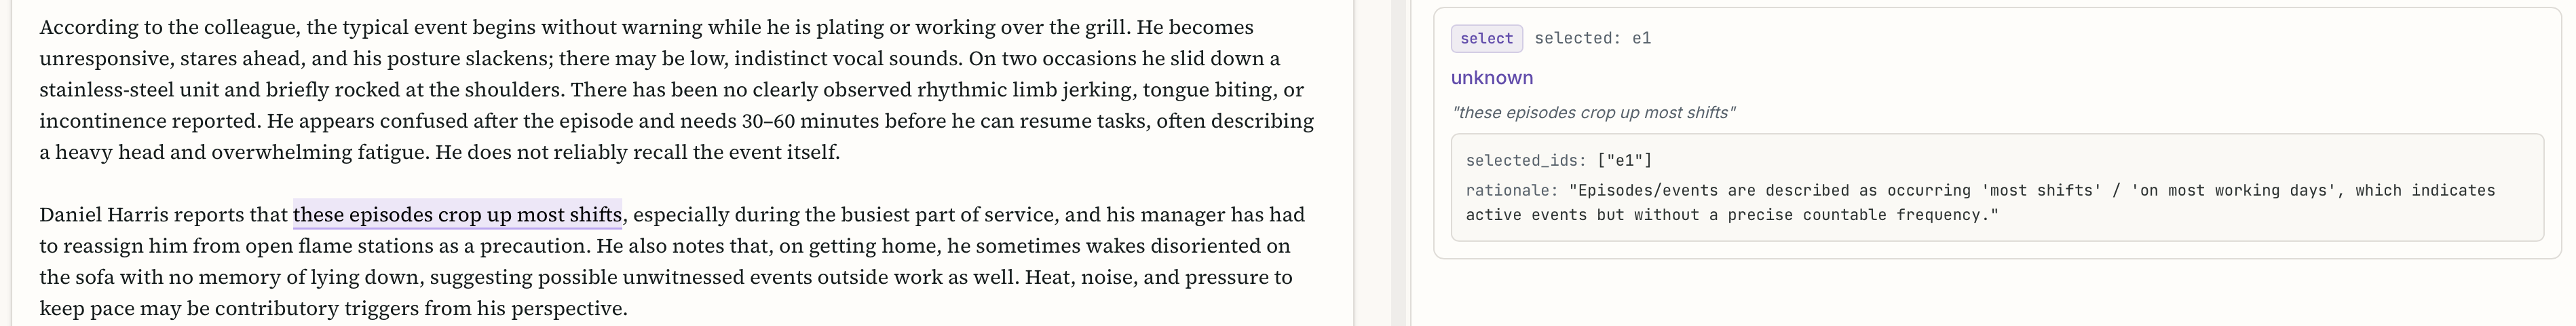
\includegraphics[width=\linewidth]{frequent_unknown1}
        \caption{Frequent $\rightarrow$ unknown (development example). Gold-standard label: multiple per week. Model selected unknown.}
        \label{fig:frequent_unknown1}
    \vspace*{4pt}
\end{figure*}

\begin{figure*}[t]
    \centering
    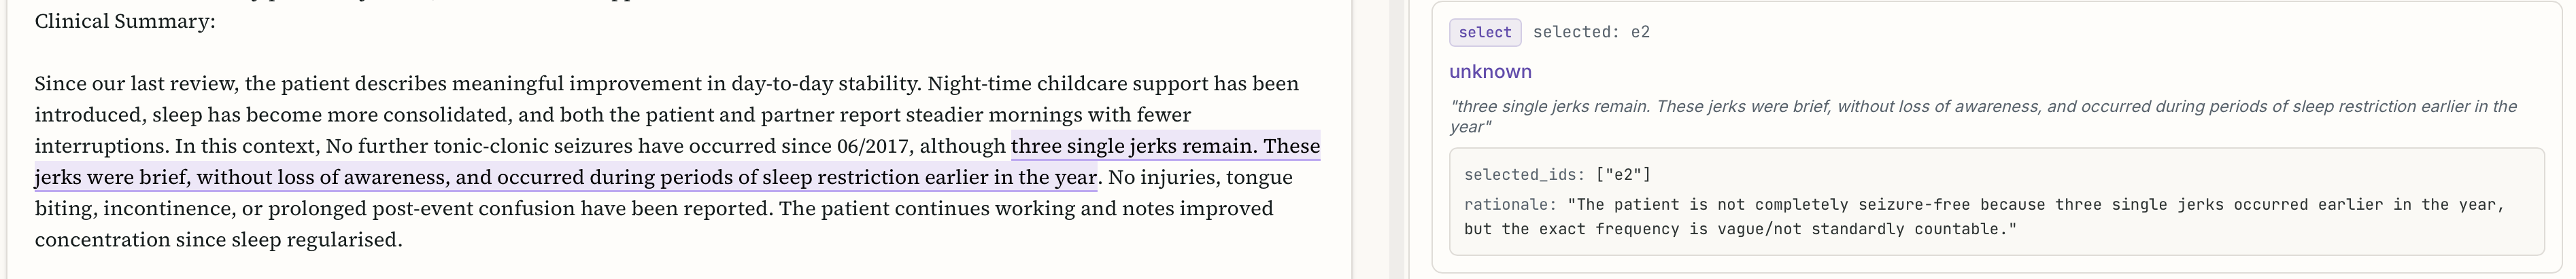
\includegraphics[width=\linewidth]{infrequent_unknown1.png}
     \caption{Infrequent $\rightarrow$ unknown (development example). Gold-standard label: 3 per 14 months. Model selected unknown.}
    \label{fig:infrequent_unknown}
\end{figure*}

\subsection{Healthcare capability index}

Figure~\ref{healthindex} plots each model's Hybrid Purist 
micro-F1 on \texttt{test450} against a published healthcare 
capability index for that model. Medical intelligence is 
closely correlated with performance in this clinical 
extraction task.

\begin{figure}[t]
    \centering
    
\includegraphics[width=\linewidth]{healthcare_index_vs_purist_f1.pdf}
    \caption{Hybrid Purist micro-F1 on Gan \texttt{test450} versus a published healthcare capability index for each extraction model. Higher index values track higher Purist stops on this synthetic task; the association is descriptive, not causal.}
    \label{healthindex}
\end{figure}

\subsection{Experimental environment}

Experiments using local language models took place on a 
Dell XPS 16 9640 running Windows 11, with an Intel Core 
Ultra 9 185H, 32 GB RAM, and an NVIDIA GeForce RTX 
4070 Laptop GPU (8 GB VRAM). Ollama v0.32.15 was 
used to serve the two local models (Qwen 3.8 27B, Gemma 4 
26B). Those local results show that the Hybrid stack can 
run on a single laptop GPU under the same synthetic task 
conditions; they are not real-letter performance, clinical 
validity, or deployment readiness.

Experiments using hosted APIs were run from a Mac 
mini M1 with 16 GB unified memory on macOS 26.5.2. API
calls were made directly to the provider (OpenAI, DeepSeek) 
or through model routers (OpenRouter, AI Gateway). Four 
hosted models were used (Gemini 3.7 Flash, GPT-5.6 Luna, 
Grok 4.6, DeepSeek V4 Flash). Hosted accelerators are not 
disclosed by the providers.

All models used a temperature of 0 except Luna, which only 
accepts a temperature of 1. An ablation was run on Gemini 
using a temperature of 1. All models used a thinking or effort 
level of low. Ablations were run on Gemini using thinking 
levels of medium and high. 

Experiments were run with Python 3.14.4. DSPy 3.2.1, 
Pydantic 2.13.4 and LiteLLM 1.87.1 were the core packages. 
DSPy co-ordinated the model calls and required structured 
JSON output. Pydantic validated that the structured output 
conformed to the schema. LiteLLM delivered API calls to Ollama 
and the model routers. Every reported cell is replayable from 
saved model output in the repository's 
\texttt{paper\_experiments/} directory without a new model 
call.

\subsection{Descriptive clinical inventory feasibility}
\label{sec:inventory-feasibility}

This task focused on one current seizure-frequency label 
per letter. The same synthetic letters also mention 
diagnoses, medicines and investigations. To show that 
broader structured content, the inventory schema and 
extraction program built for the separate ExECTv2 
task~\cite{b3} was applied to a sample of 100 letters
in this dataset. Summary results are in Table~\ref{tab:inventory}.
An example of an annotated letter is shown in Figure~\ref{inventory_demo}.

\begin{table*}[!t]
\caption{Descriptive inventory output on 100 \texttt{dev750} synthetic letters.}
\label{tab:inventory}
\centering
\footnotesize
\begin{tabularx}{\textwidth}{lrrlY}
\toprule
\textbf{Family} & \textbf{Letters $\geq$1} & \textbf{Facts} & \textbf{Median (range)} & \textbf{Common named types} \\
\midrule
Diagnosis & 76 & 130 & 1 (0--4) & epilepsy, focal epilepsy, generalised epilepsy, secondary generalised seizures, generalised seizures \\
Prescription & 81 & 204 & 2 (0--9) & levetiracetam, lamotrigine, sodium valproate, clobazam, topiramate \\
Investigations & 40 & 68 & 0 (0--3) & MRI normal, EEG abnormal, EEG normal, MRI abnormal \\
Any reported family & 93 & 402 & 4 (0--11) & --- \\
\bottomrule
\end{tabularx}
\end{table*}

\begin{figure}[t]
    \centering
    
\includegraphics[width=\linewidth]{inventory.png}
    \caption{Example of extracting multiple entities from the letter in a broader clinical inventory using the ExECT schema.}
    \label{inventory_demo}
\end{figure}

\section{Tools}

\subsection{Development environment and implementation}

The implementation used Python (version 3.11 or later), which provided one
language for data loading, deterministic extraction rules, experiment
orchestration, and evaluation. DSPy supplied the structured interface for
language-model programs and their typed inputs and outputs. LiteLLM provided
a common model-access layer across hosted providers and the local Ollama
route, allowing the experiment code to retain the same orchestration pattern
while changing the model endpoint. Pydantic was used for explicit data
models and validation, helping keep intermediate records and experiment
configuration machine-readable. 

\subsection{Model access and inference infrastructure}

Hosted models were accessed through provider APIs, with DSPy and LiteLLM
handling the shared calling interface, request settings, timeouts, and retry
behaviour. This made it possible to compare several providers within the
same experiment design without treating their serving hardware as part of
the local development environment. 

The local open-weight models used in the reported extracts were served with
native Ollama chat at \texttt{http://localhost:11434}. In particular, Qwen
3.8 27B and Gemma 4 26B used the \texttt{ollama\_chat/...} route. 

\subsection{Verification, testing, and reproducibility}

Pytest provided automated checks for the extraction pipeline and its data
handling. Ruff checked Python style and common implementation errors, while
mypy checked the consistency of annotated interfaces. Together these tools
supported the implementation and testing stages by detecting regressions
before experiments were run. 

Reproducibility was supported by the dependency declaration and lockfile,
prespecified model routes and request settings, and per-cell experiment
artifacts retaining the prompt or program version, split, scorer, and retry
settings. 

The assessed code repository is on QUB EEECS
GitLab at \url{https://gitlab.eeecs.qub.ac.uk/40466218/clinical_extraction.git}.

\section{Critical Appraisal}

\subsection{Successes}

The project produced a reproducible pipeline for extracting a
single current seizure-frequency label from synthetic epilepsy clinic letters.
Its main contribution was to separate the task into two inspectable stages:
an LLM extracted candidate evidence into a structured record, and a decision
stage returned the final label. Holding the extraction record fixed made it
possible to compare a rules-based system with a second LLM call. Empirical
analysis demonstrated that the \texttt{Hybrid} method performed better under 
all conditions tested, particularly for smaller models more likely to be deployed
on hospital servers.

The pipeline showed consistent performance on the synthetic data (0.83/0.77)
and test (0.8/0.77) and the external test set of 300 real patient letters, demonstrating 
both the \texttt{Hybrid} / 0.77 \texttt{LLM-Only} methods are robust. The original
research objective was an empirical study of reliability, and this is the strongest
signal of reliability.

The most important design decision was to narrow the dissertation to the
seizure frequency task. The original project explored both Gan and ExECTv2,
but the two datasets have different annotation policies, outcome definitions,
scorers, and error profiles. Presenting both as equal dissertation results
would have required the reader to work too hard. Narrowing the results 
produced a cleaner argument and provided more room to demonstrate the
methodology. 

\subsection{Limitations and challenges}

The main limitation is the primary data source used. A single model (DeepSeek)
was run on an external test set of patient data and showed strong transfer, but all other 
evaluations in the research used synthetic data. Synthetic data has been shown
to produce more positive results in prior papers as it contains fewer typos, 
idiosyncrasies and a more consistent structure than real data. Past results have also
shown that performance on once corpus of real patient data are not evidence that
they will translate to other hospital templates or clinician writing styles. Thus, 
the results are promising but must be interpreted within those boundaries.

The secondary limitation is the lack of evidence that the method transfers to
other tasks. The ExECTv2 work was designed to illustrate that the same methods
can be applied to a task that requires a much richer schema: multiple clinical 
categories, multiple entities per category and multiple attributes per entity, vs.
the single-label extraction task demonstrated here. That must be demonstrated 
in future work to show the two-stage extraction pipeline architecture generalises
beyond a very specific task design.

\subsection{Lessons learned and future work}

The main lesson learned is that there is no substitute for examining the data
in depth. Early experiments were run with a focus on the high-level metrics:
precision, recall, F1 score. Iterations of prompt engineering and rule design 
would improve performance in one area and harm it in another. When
I started to look in depth at the 400-word clinic letters themselves, the predictions
the model made and, most importantly, the gold-standard annotations, it became
clear that the complicated part of the task was a highly specific decision policy
to choose the right answer. However, I avoided doing that early on because the
letters were long, dense and the annotations were on a subject I lacked domain
expertise in. Building a deeper understanding of what the data represented
made the architecture design and optimisation process much simpler.

The next step is evaluate whether the pipeline has clinical value. This should include 
expert review of whether the cited evidence supports the selected label, and
prospective assessment of how clinicians would use or contest the outputs.
The independent real-letter scores already show that the package can be
run and scored outside the development environment; they do not replace
those studies. Those studies would need their own data-access, ethics, and
validation decisions. Until then, the system can only be presented as a
reproducible research prototype rather than a clinical decision tool.

\begin{thebibliography}{00}

\bibitem{b1} S.~T. Rosenbloom, J.~C. Denny, H. Xu, N. Lorenzi, W.~W. Stead, and K.~B. Johnson, ``Data from clinical notes: A perspective on the tension between structure and flexible documentation,'' \emph{J. Amer. Med. Informat. Assoc.}, vol.~18, no.~2, pp.~181--186, 2011.
\bibitem{b2} D.~A. Hanauer, Y. Liu, Q. Mei, F.~J. Manion, U.~J. Balis, and K. Zheng, ``Hedging their Mets: The use of uncertainty terms in clinical documents and its potential implications when sharing the documents with patients,'' in \emph{AMIA Annu. Symp. Proc.}, 2012, pp.~321--330.
\bibitem{b3} B. Fonferko-Shadrach \emph{et al.}, ``Annotation of epilepsy clinic letters for natural language processing,'' \emph{J. Biomed. Semantics}, vol.~15, no.~17, 2024.
\bibitem{b4} B. Fonferko-Shadrach \emph{et al.}, ``Using natural language processing to extract structured epilepsy data from unstructured clinic letters: development and validation of the ExECT (extraction of epilepsy clinical text) system,'' \emph{BMJ Open}, vol.~9, no.~4, 2019, Art.~no.~e023232.
\bibitem{b5} Y. Gan \emph{et al.}, ``Reproducible synthetic clinical letters for seizure frequency information extraction,'' arXiv:2603.11407, 2026.
\bibitem{b6} K. Xie \emph{et al.}, ``Extracting seizure frequency from epilepsy clinic notes: a machine reading approach to natural language processing,'' \emph{J. Amer. Med. Informat. Assoc.}, vol.~29, no.~5, pp.~873--881, 2022.
\bibitem{b7} B. Holgate, S. Fang, A. Shek, M. McWilliam, P. Viana, J.~S. Winston, J.~T. Teo, and M.~P. Richardson, ``Extracting epilepsy patient data with Llama 2,'' in \emph{Proc. 23rd Workshop on Biomedical Natural Language Processing (BioNLP)}, 2024, pp.~526--535.
\bibitem{b8} B. Holgate, J. Davies, S. Fang, J.~S. Winston, J.~T. Teo, and M.~P. Richardson, ``Fine-tuning LLMs to extract epilepsy seizure frequency data from health records,'' in \emph{Proc. 24th Workshop on Biomedical Language Processing (BioNLP)}, 2025, pp.~44--55.
\bibitem{b9} B.~M. Decker \emph{et al.}, ``Development of a natural language processing algorithm to extract seizure types and frequencies from the electronic health record,'' \emph{Seizure}, vol.~101, pp.~48--51, 2022.
\bibitem{b10} M. Fernandes, A. Cardall, L.~M.~V.~R. Moura, C. McGraw, S.~F. Zafar, and M.~B. Westover, ``Extracting seizure control metrics from clinic notes of patients with epilepsy: A natural language processing approach,'' \emph{Epilepsy Res.}, vol.~207, 2024, Art.~no.~107451.
\bibitem{b11} T. Brown \emph{et al.}, ``Language models are few-shot learners,'' in \emph{Adv. Neural Inf. Process. Syst. (NeurIPS)}, vol.~33, 2020, pp.~1877--1901.
\bibitem{b12} M. Agrawal, S. Hegselmann, H. Lang, Y. Kim, and D. Sontag, ``Large language models are few-shot clinical information extractors,'' in \emph{Proc. Conf. Empirical Methods in Natural Language Processing (EMNLP)}, 2022, pp.~1998--2022.
\bibitem{b13} R. Grishman and B. Sundheim, ``Message Understanding Conference-6: A brief history,'' in \emph{Proc. 16th Int. Conf. Computational Linguistics (COLING)}, 1996, pp.~466--471.
\bibitem{b14} Z. Yang \emph{et al.}, ``CLINES: Clinical LLM-based information extraction and structuring agent,'' medRxiv:10.64898/2025.12.01.25341355, 2025.
\bibitem{b15} S. Fang, B. Holgate, A. Shek, J.~S. Winston, M. McWilliam, P.~F. Viana, J.~T. Teo, and M.~P. Richardson, ``Extracting epilepsy-related information from unstructured clinic letters using large language models,'' \emph{Epilepsia}, vol.~66, pp.~3369--3384, 2025.
\bibitem{b16} S. Wigglesworth, A. Neligan, J.~M. Dickson, A. Pullen, E. Yelland, T. Anjuman, and M. Reuber, ``The incidence and prevalence of epilepsy in the United Kingdom 2013--2018: A retrospective cohort study of UK primary care data,'' \emph{Seizure}, vol.~105, pp.~37--42, 2023.
\bibitem{b17} R.~S. Fisher \emph{et al.}, ``ILAE official report: A practical clinical definition of epilepsy,'' \emph{Epilepsia}, vol.~55, no.~4, pp.~475--482, 2014.
\bibitem{b18} K. Xie, B. Litt, D. Roth, and C.~A. Ellis, ``Quantifying clinical outcome measures in patients with epilepsy using the electronic health record,'' in \emph{Proc. BioNLP Workshop}, 2022, pp.~369--375.
\bibitem{b19} L. Cui, S.~S. Sahoo, S.~D. Lhatoo, G. Garg, P. Rai, A. Bozorgi, and G.-Q. Zhang, ``Complex epilepsy phenotype extraction from narrative clinical discharge summaries,'' \emph{J. Biomed. Informat.}, vol.~51, pp.~272--279, 2014.
\bibitem{b20} S. Fu \emph{et al.}, ``Clinical concept extraction: A methodology review,'' \emph{J. Biomed. Informat.}, vol.~109, 2020, Art.~no.~103526.
\bibitem{b21} Y. Wang \emph{et al.}, ``Clinical information extraction applications: A literature review,'' \emph{J. Biomed. Informat.}, vol.~77, pp.~34--49, 2018.
\bibitem{b22} L. Chiticariu, Y. Li, and F. Reiss, ``Rule-based information extraction is dead! Long live rule-based information extraction systems!,'' in \emph{Proc. Conf. Empirical Methods in Natural Language Processing (EMNLP)}, 2013, pp.~827--832.
\bibitem{b23} R.~E. Sherman \emph{et al.}, ``Real-world evidence---what is it and what can it tell us?'' \emph{N. Engl. J. Med.}, vol.~375, no.~23, pp.~2293--2297, 2016.
\bibitem{b24} J. Wang \emph{et al.}, ``Scaling clinician-grade feature generation from clinical notes with multi-agent language models,'' arXiv:2508.01956, 2025.
\bibitem{b25} A. Gorenshtein et. al, AI Agents in Clinical Medicine: A Systematic Review
\bibitem{b26} D. Tran, Single-Agent LLMs Outperform Multi-Agent Systems on Multi-Hop Reasoning Under Equal Thinking Token Budgets

\end{thebibliography}

\section{Appendices}
\subsection{Appendix 1: LLM prompt used in the extract stage}
\lstinputlisting{gan_llm_extract_prompt_template.json}

\end{document}
